% Drawing 144/09-1 -- folder 144, batch 09, archive page 161 (PDF page 162).
% Transcription: à gauche, un parallélépipède en pointillés, flèches le long des arêtes ; au centre, un cylindre (anneau) avec deux arcs $X'$ (en dessus) et $X''$ (le long du cylindre), les points $a_0, a_1, a_2, a_3$, deux vecteurs $e'$, $e''$ issus de $a_0$ et une flèche de rotation $\sigma$ ; au-dessus, une petite croix fléchée.
% Kind: dotted parallelepiped; ring with arcs X', X'', frame e', e'' and rotation sigma. Method 2 (schematic redraw from the facsimile). Status: partial.
% Notes: Re-read on a tight crop of the upright page. Left: the parallelepiped, its eight corners placed once and every edge drawn between them in the stroke he uses (dashed edges with the arrowheads he draws, the two heavily dotted edges at the front left, faint pencil edges), the inner rectangle in dashed strokes with its arrows, and the three loose arrows inside. Right: the ring lying on its side (left end dashed, right end solid, bottom line X''), the two dashed arcs of X' over it with their arrowheads, the points a_3, a_0, a_2, a_1, the two vectors from a_0 (e' along the ring, the upward one thick), e'' labelled, the small rotation arrow under a_0 labelled sigma, the thick curved arrow at the right end; above, the small crossed arrows between two arcs. Labels \small. Still differs from the facsimile: the arcs of the ring are overinked and approximate; e'' sits by a curved arrow that is not drawn separately; the label sigma is placed after the transcription (the sign on the page is not legible); the crossed arrows at the top are a reading. The formulas below are text. Redrawn 2026-11-09 (issue 128): to check again. Overlay check 2026-11-13 (issue 147, Claude Opus 5.5): the redraw, rasterised from its TikZ paths, laid over the 300 dpi colour render of the 250 ppi scan with the contrast raised: the parallelepiped (corners, dashed and dotted edges, the inner rectangle and the loose arrows) lies on its ink to within about 1 unit; on the ring the overinked arcs are within 1 to 2 units. Nothing changed. Still differs, as listed above: the arcs of the ring are overinked and approximate; e'' sits by a curved arrow not drawn separately; the label sigma is placed after the transcription (the sign is not legible); the crossed arrows at the top are a reading. Not compiled (no TeX engine in the session).
% Coordinates: 1 unit = 1 mm = 1/100 of the crop width (bbox in page fractions: [0.1, 0.09, 0.52, 0.3]).
% Redrawn by Claude (claude-opus-5-5), issue #73, 2026-11-09; not checked by a human; not compiled (no TeX in the session).
% Checked by Claude (claude-opus-5-5) 2026-11-13 (issue #147): overlay on the 300 dpi colour render of the 250 ppi scan; nothing changed; not compiled (no TeX in the session). Not checked by a human. Status: partial.
% Rights: reproduces part of the work -- behind RENDER_TRANSCRIPTS, never published by itself.
\documentclass[tikz,border=3pt]{standalone}
\usepackage{amsmath,amssymb}
\usetikzlibrary{patterns,arrows.meta}
\tikzset{pencil/.style={black!45}, struck/.style={black!35}, mark/.style={circle,draw,inner sep=1.3pt}, pt/.style={circle,fill,inner sep=0.9pt}, opt/.style={circle,draw,fill=white,inner sep=1.1pt}}
\begin{document}
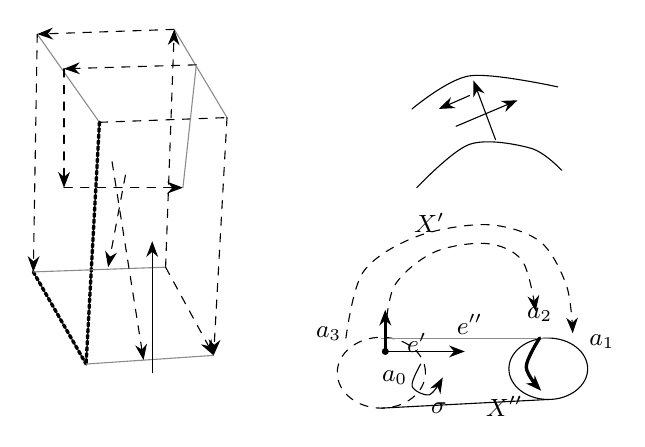
\begin{tikzpicture}[x=1mm,y=1mm,line cap=round,line join=round,font=\scriptsize]
\draw[dashed,-{Stealth[length=2mm]}] (36.1,-6.7) -- (18.7,-7.3);
\draw[pencil] (36.1,-6.7) -- (42.8,-17.9);
\draw[dashed] (26.6,-18.5) -- (42.8,-17.9);
\draw[pencil] (18.7,-7.3) -- (26.6,-18.5);
\draw[dashed,-{Stealth[length=2mm]}] (18.7,-7.3) -- (18.2,-37.5);
\draw[densely dotted,very thick] (26.6,-18.5) -- (24.9,-49.2);
\draw[dashed,-{Stealth[length=2mm]}] (35,-36.9) -- (36.1,-6.7);
\draw[dashed,-{Stealth[length=2mm]}] (42.8,-17.9) -- (41.1,-48.1);
\draw[densely dotted,very thick] (18.2,-37.5) -- (24.9,-49.2);
\draw[pencil] (24.9,-49.2) -- (41.1,-48.1);
\draw[pencil] (18.2,-37.5) -- (35,-36.9);
\draw[dashed,-{Stealth[length=2mm]}] (35,-36.9) -- (41.1,-48.1);
\draw[dashed,-{Stealth[length=2mm]}] (38.9,-11.2) -- (22.1,-11.7);
\draw[dashed,-{Stealth[length=2mm]}] (22.1,-11.7) -- (22.1,-26.8);
\draw[dashed,-{Stealth[length=2mm]}] (22.1,-26.8) -- (37.2,-26.8);
\draw[pencil] (38.9,-11.2) -- (37.2,-26.8);
\draw[dashed,-{Stealth[length=2mm]}] (28.2,-23.5) -- (32.2,-48.7);
\draw[dashed,-{Stealth[length=2mm]}] (29.9,-25.2) -- (27.7,-36.9);
\draw[-{Stealth[length=2mm]}] (33.3,-50.3) -- (33.3,-33.6);
\draw[dashed] (62.4,-50.3) ellipse[x radius=5.6, y radius=4.5];
\draw (83.6,-49.8) ellipse[x radius=5, y radius=3.9];
\draw (62.4,-54.8) -- (83.6,-53.7);
\draw[pencil] (62.4,-45.9) -- (83.6,-45.9);
\draw[dashed,-{Stealth[length=2mm]}] plot[smooth, tension=0.55] coordinates {(57.9,-45.9) (60.1,-37.5) (66.9,-33) (75.8,-31.5) (82.5,-33.6) (85.9,-39.2) (86.7,-45.3)};
\draw[dashed,-{Stealth[length=2mm]}] plot[smooth, tension=0.55] coordinates {(62.9,-45.3) (64.1,-39.2) (69.1,-35) (75.8,-33.9) (80.3,-36.1) (82,-42.5)};
\draw[-{Stealth[length=2mm]},very thick] (62.9,-47.6) -- (62.9,-42.3);
\draw[-{Stealth[length=2mm]}] (62.9,-47.6) -- (73,-47.6);
\draw[-{Stealth[length=2mm]}] plot[smooth, tension=0.55] coordinates {(67.4,-49.2) (66.3,-52) (68.5,-53.1) (70.2,-50.9)};
\draw[-{Stealth[length=2mm]},very thick] plot[smooth, tension=0.55] coordinates {(82.5,-45.9) (80.8,-49.6) (82.7,-52.6)};
\draw plot[smooth, tension=0.55] coordinates {(66.3,-16.8) (73.6,-12.6) (84.8,-14)};
\draw plot[smooth, tension=0.55] coordinates {(66.9,-26.8) (73.6,-21.3) (81.4,-21.8) (85.3,-24.6)};
\draw[-{Stealth[length=2mm]}] (71.9,-19) -- (79.7,-15.7);
\draw[-{Stealth[length=2mm]}] (76.9,-20.7) -- (74.1,-13.2);
\draw[-{Stealth[length=2mm]}] (73.6,-15.1) -- (69.7,-16.8);
\node[pt] at (62.9,-47.6) {};
\node[inner sep=1pt] at (55.7,-45.3) {\small $a_3$};
\node[inner sep=1pt] at (64.1,-50.9) {\small $a_0$};
\node[inner sep=1pt] at (82.5,-42.9) {\small $a_2$};
\node[inner sep=1pt] at (90.4,-46.4) {\small $a_1$};
\node[inner sep=1pt] at (66.9,-46.5) {\small $e'$};
\node[inner sep=1pt] at (73.6,-44.2) {\small $e''$};
\node[inner sep=1pt] at (68.5,-31.3) {\small $X'$};
\node[inner sep=1pt] at (78,-54.6) {\small $X''$};
\node[inner sep=1pt] at (69.7,-54.8) {\small $\sigma$};
\end{tikzpicture}
\end{document}
